%%%%%%%%%%%%%%%%%% ATLAS

\section{The ATLAS Experiment}
\label{sed:cern:atlas}

ATLAS (A Toroidal LHC ApparatuS)\cite{atlas:atlas}

\begin{figure}[ht]
\centering
\subfigure{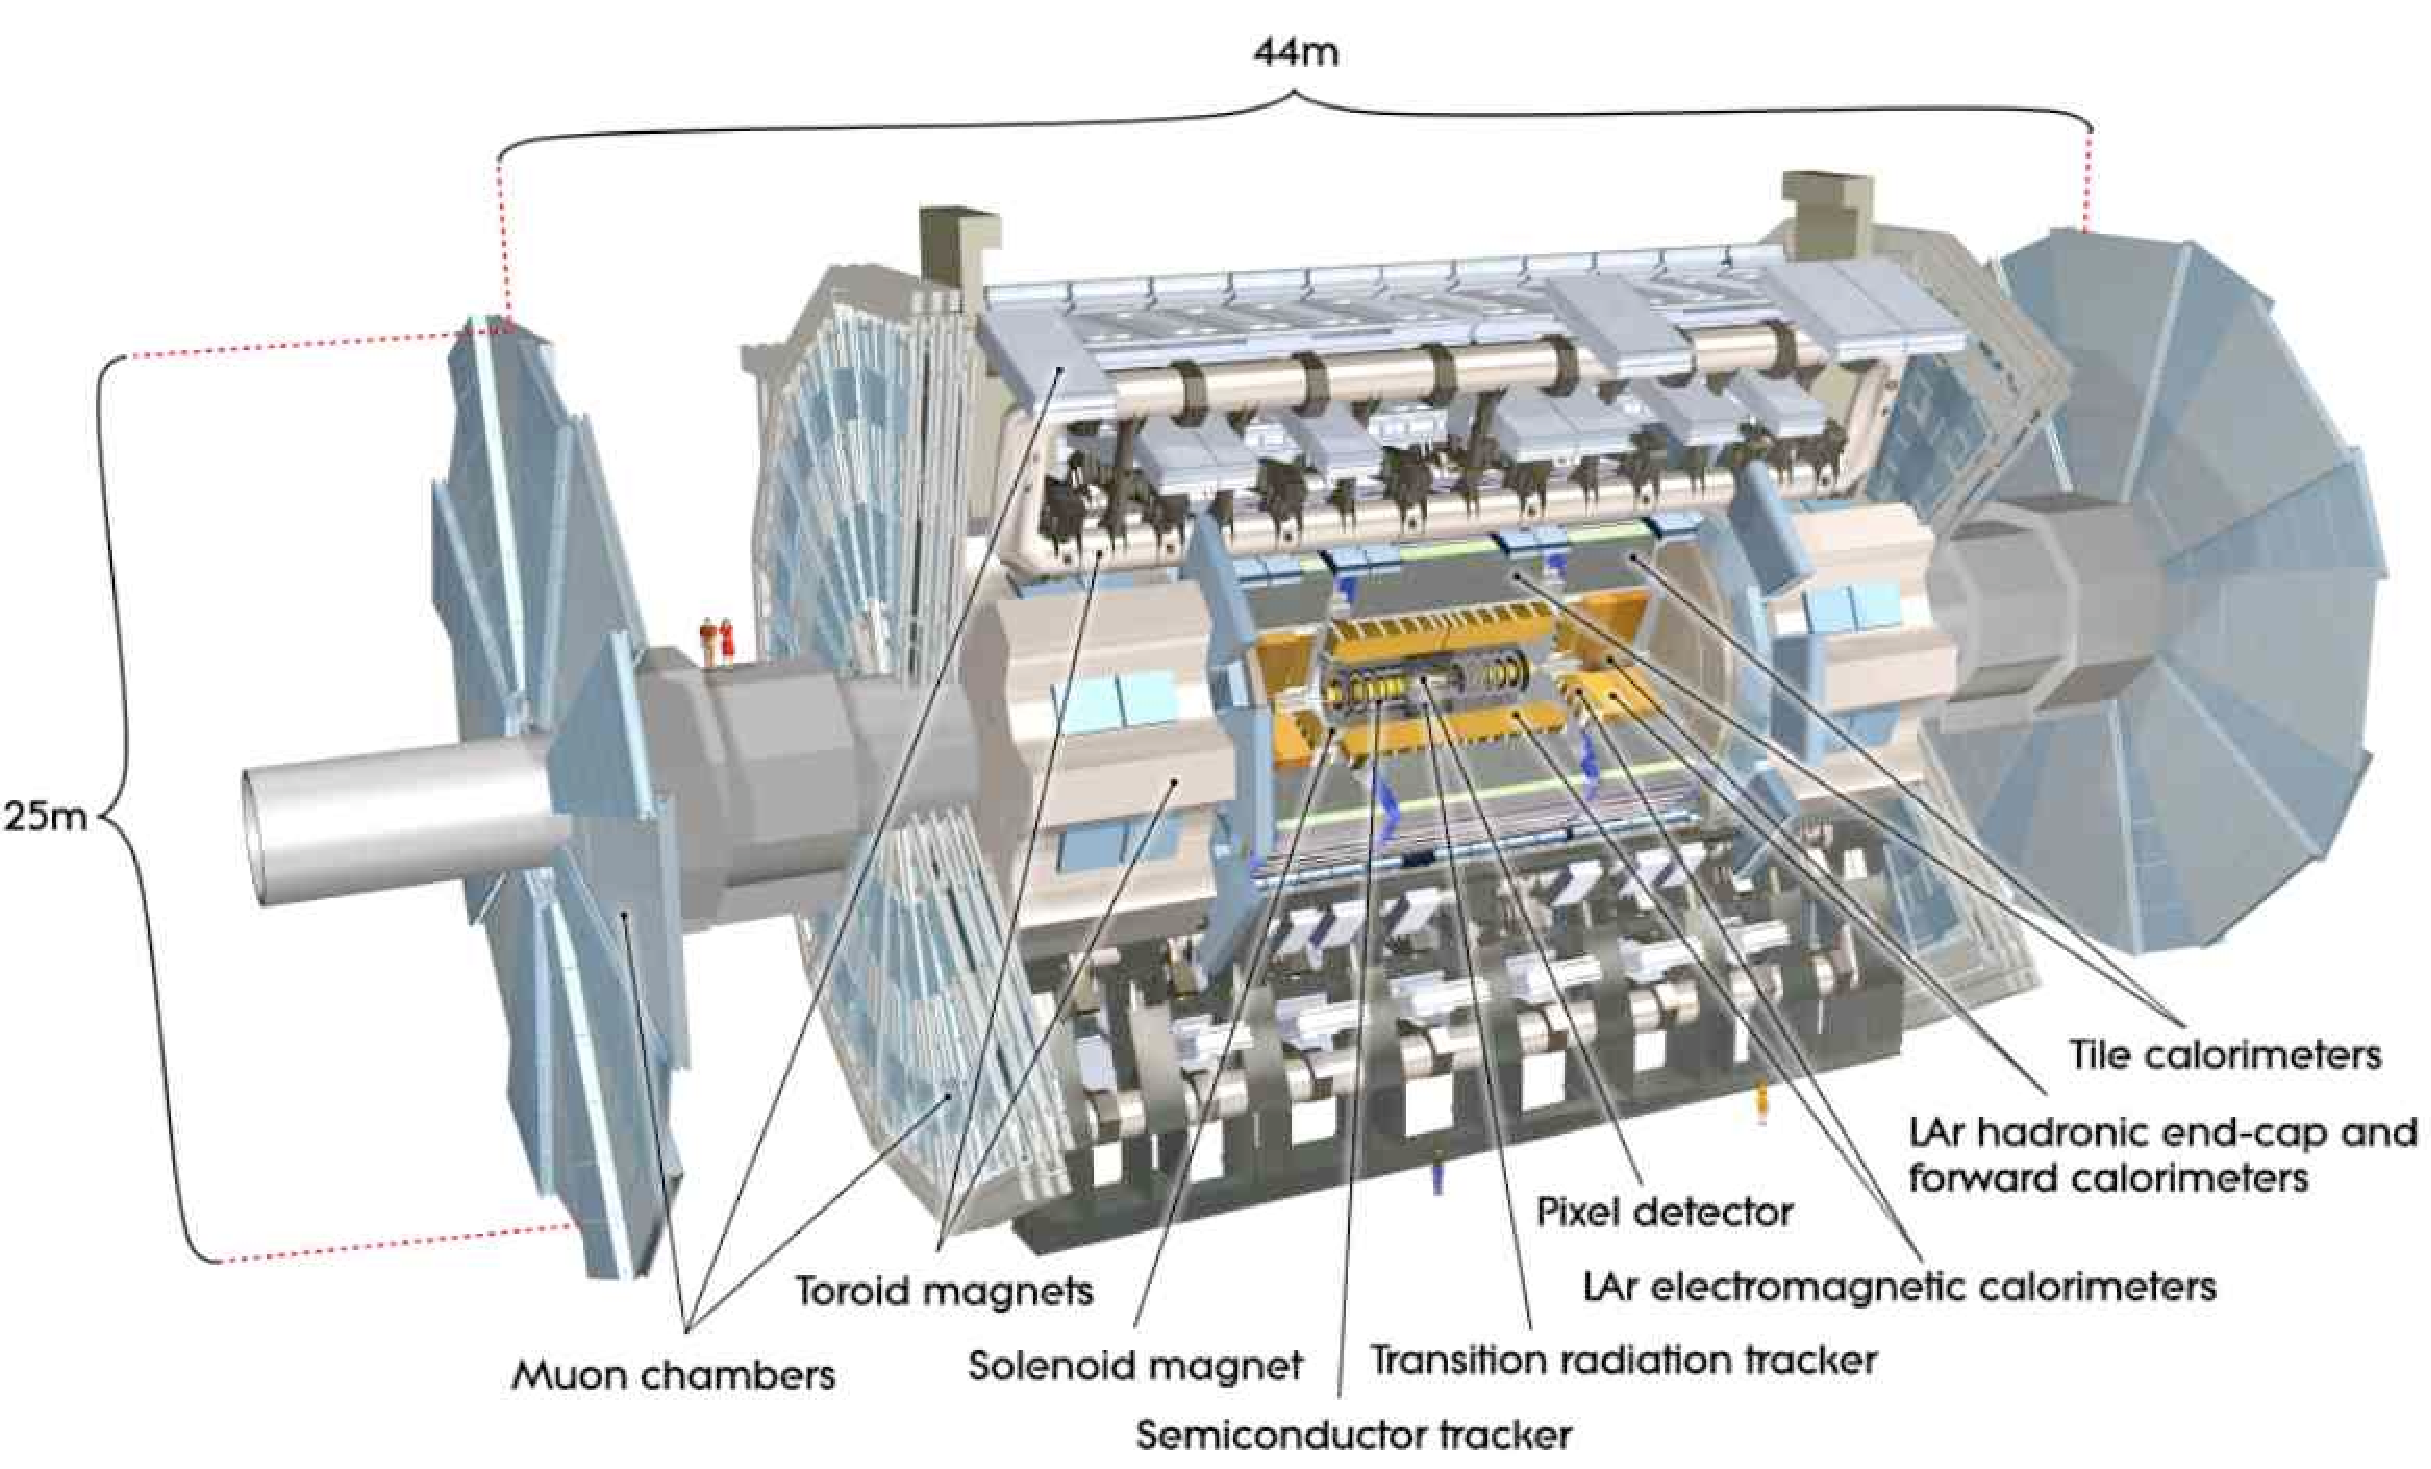
\includegraphics[width=0.85\textwidth]{figures/atlas/atlas}}
\caption{Layout of the ATLAS inner detector. Figure from Ref. \cite{atlas:atlas}}
\label{fig:atlas:atlas}
\end{figure}

\subsection{Coordinate System}

ATLAS uses a right-handed coordinate system, with its origin at the nominal interaction point. The $z$-axis follows the beam direction, while in the transverse plane the $y$-axis points upward and the $x$axis toward the LHC center. Positive and negative values of the $z$-axis identify respectively the A-side and the C-side of the detector. When spherical coordinates are used, the \textit{azimuthal angle} $\phi$ is defined starting from the $x$-axis, and ranges between $-\pi$ and $\pi$; the \textit{polar angle} $\theta$ is defined starting from the $z$-axis and takes values between $0$ and $\pi$. Often the polar angle is substituted by the \textit{pseudorapidity}: 
 
\begin{equation}
\label{eq:cern:eta}
\eta = - \ln \tan \frac{\theta}{2}
\end{equation}

which, in the limit of massless particles, is equivalent to the \textit{rapidity}:

\begin{equation}
\label{eq:cern:y}
y = \frac{1}{2} \ln \frac{E + p_z}{E - p_z} \; ,
\end{equation}

where $E$ is the energy of the particle and $p_z$ its momentum projected on the $z$-axis. The $\eta$-$\phi$ plane is used to define the angular separation of two objects in the detector:

\begin{equation}
\label{eq:cern:dR}
\Delta R = \sqrt{ \Delta \phi^2 + \Delta \eta^2  } \; .
\end{equation}

\begin{equation}
\label{eq:cern:pt}
p_T = \sqrt{p_x^2 + p_y^2}
\end{equation}

\begin{equation}
\label{eq:cern:pz}
p_z = p_T \,\sinh \eta
\end{equation}






\subsection{Magnet System}

\label{sec:cern:atlasmagnets}
\begin{figure}[ht]
\centering
\subfigure{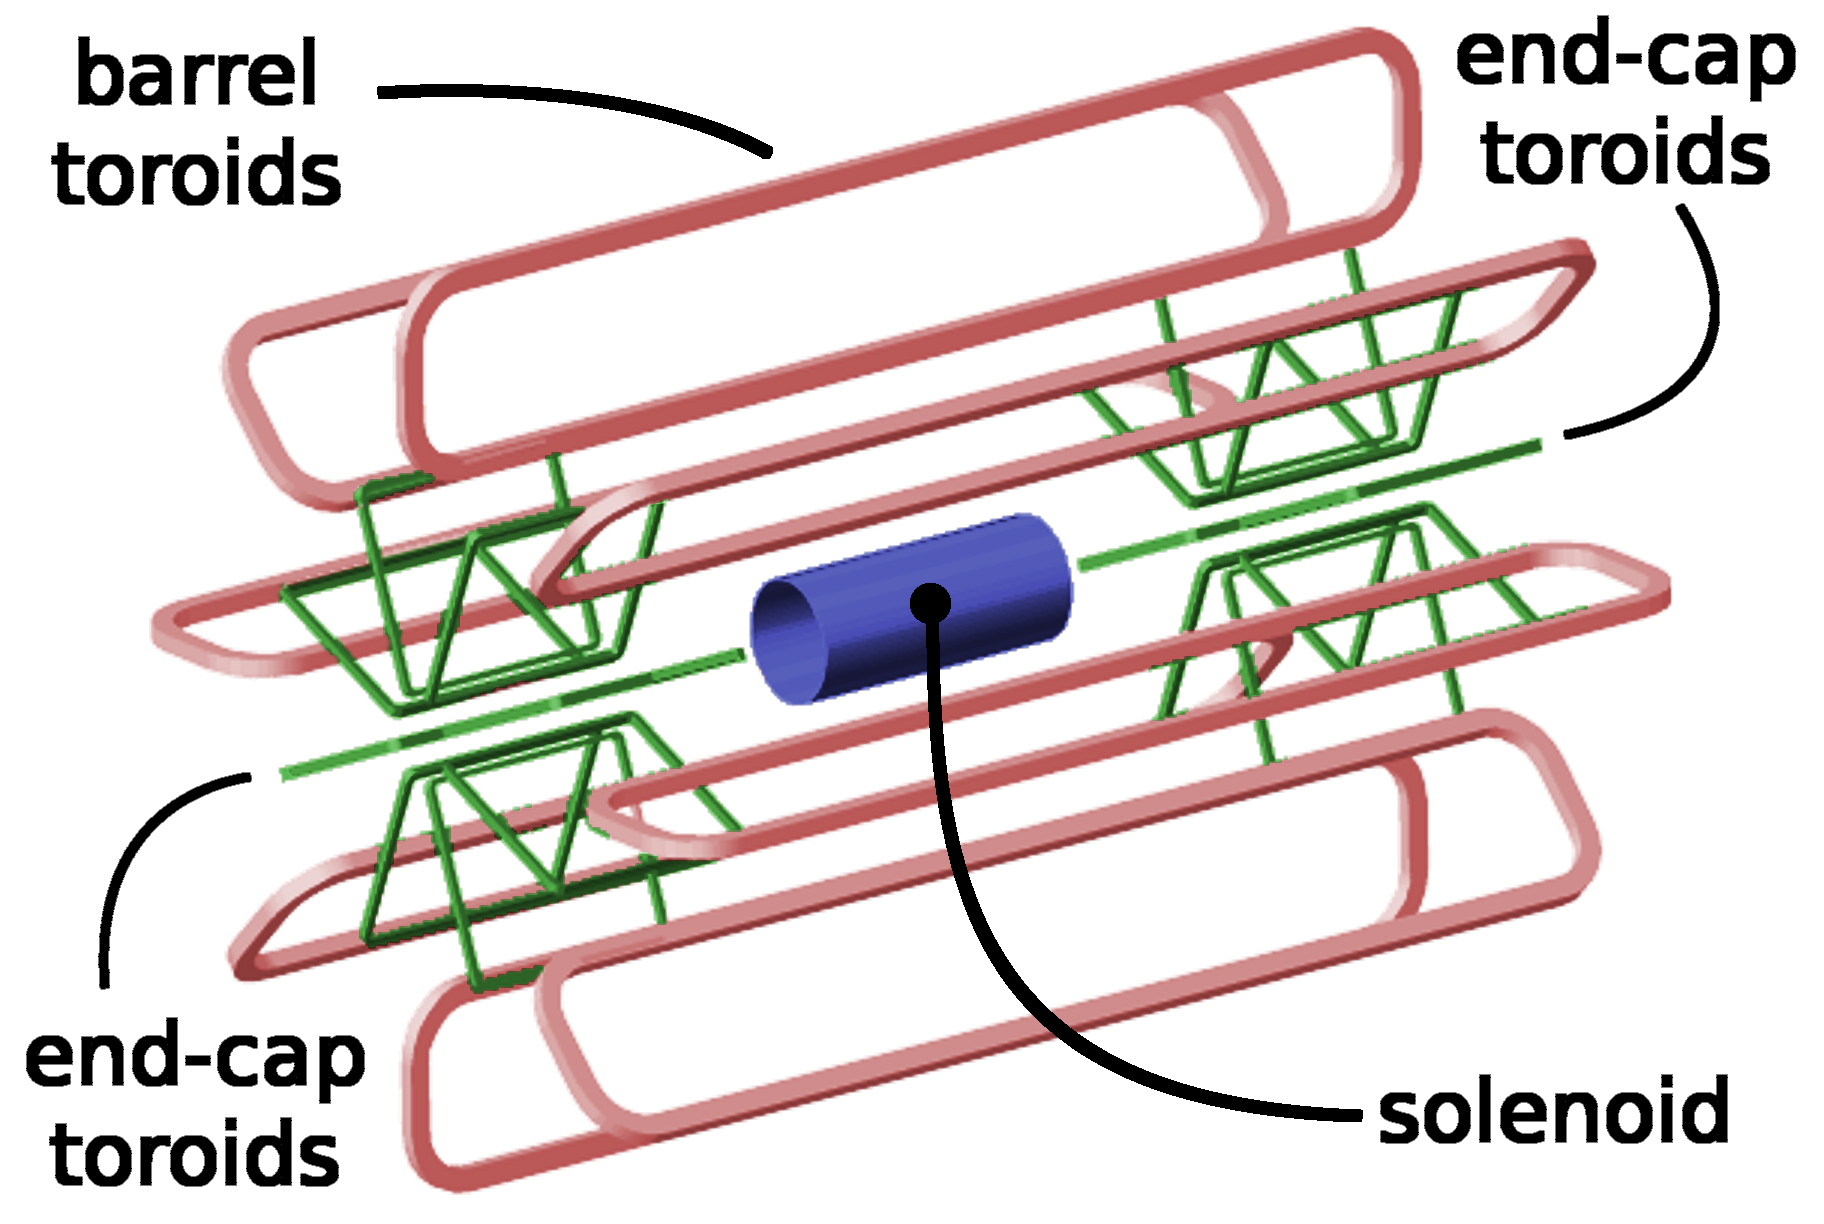
\includegraphics[width=0.35\textwidth]{figures/atlas/magnets}}
\caption{Layout of the ATLAS magnet system. Figure from Ref. \cite{Goodson}}
\label{fig:atlas:magnet}
\end{figure}



\subsubsection*{Solenoid}

\subsubsection*{Toroids}



\subsection{Inner Detector}

\begin{figure}[ht]
\centering
\subfigure{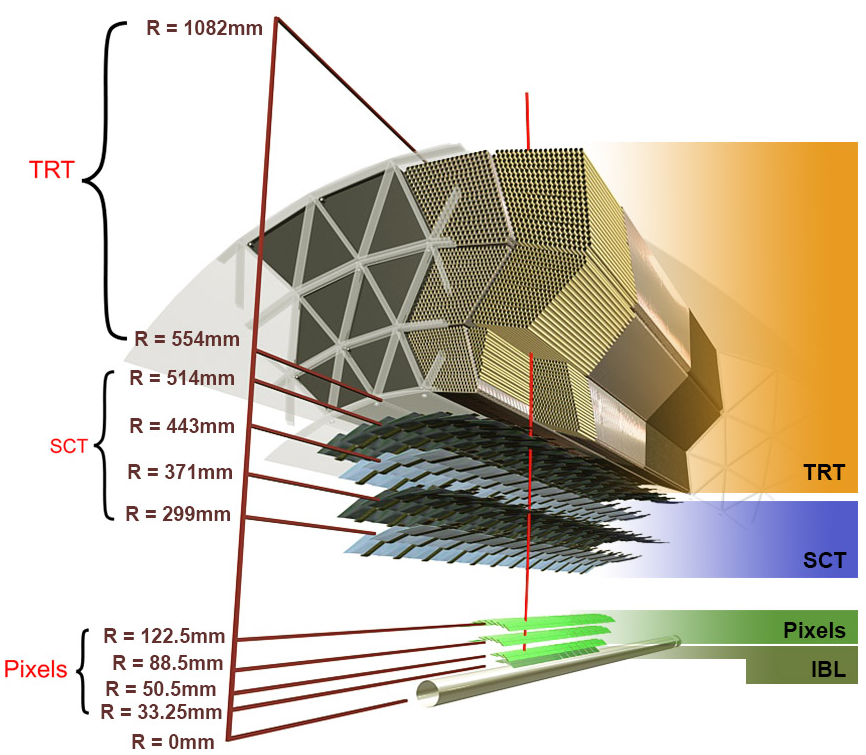
\includegraphics[width=0.65\textwidth]{figures/atlas/inner_detector}}
\caption{Layout of the ATLAS inner detector. Figure from Ref. \cite{Potamianos:2016ptf}}
\label{fig:atlas:id}
\end{figure}


\subsubsection*{Pixel Detector}


\subsubsection*{Semi-Conductor Tracker}


\subsubsection*{Transition Radiation Tracker}



\subsection{Calorimeters}

\begin{figure}[ht]
\centering
\subfigure{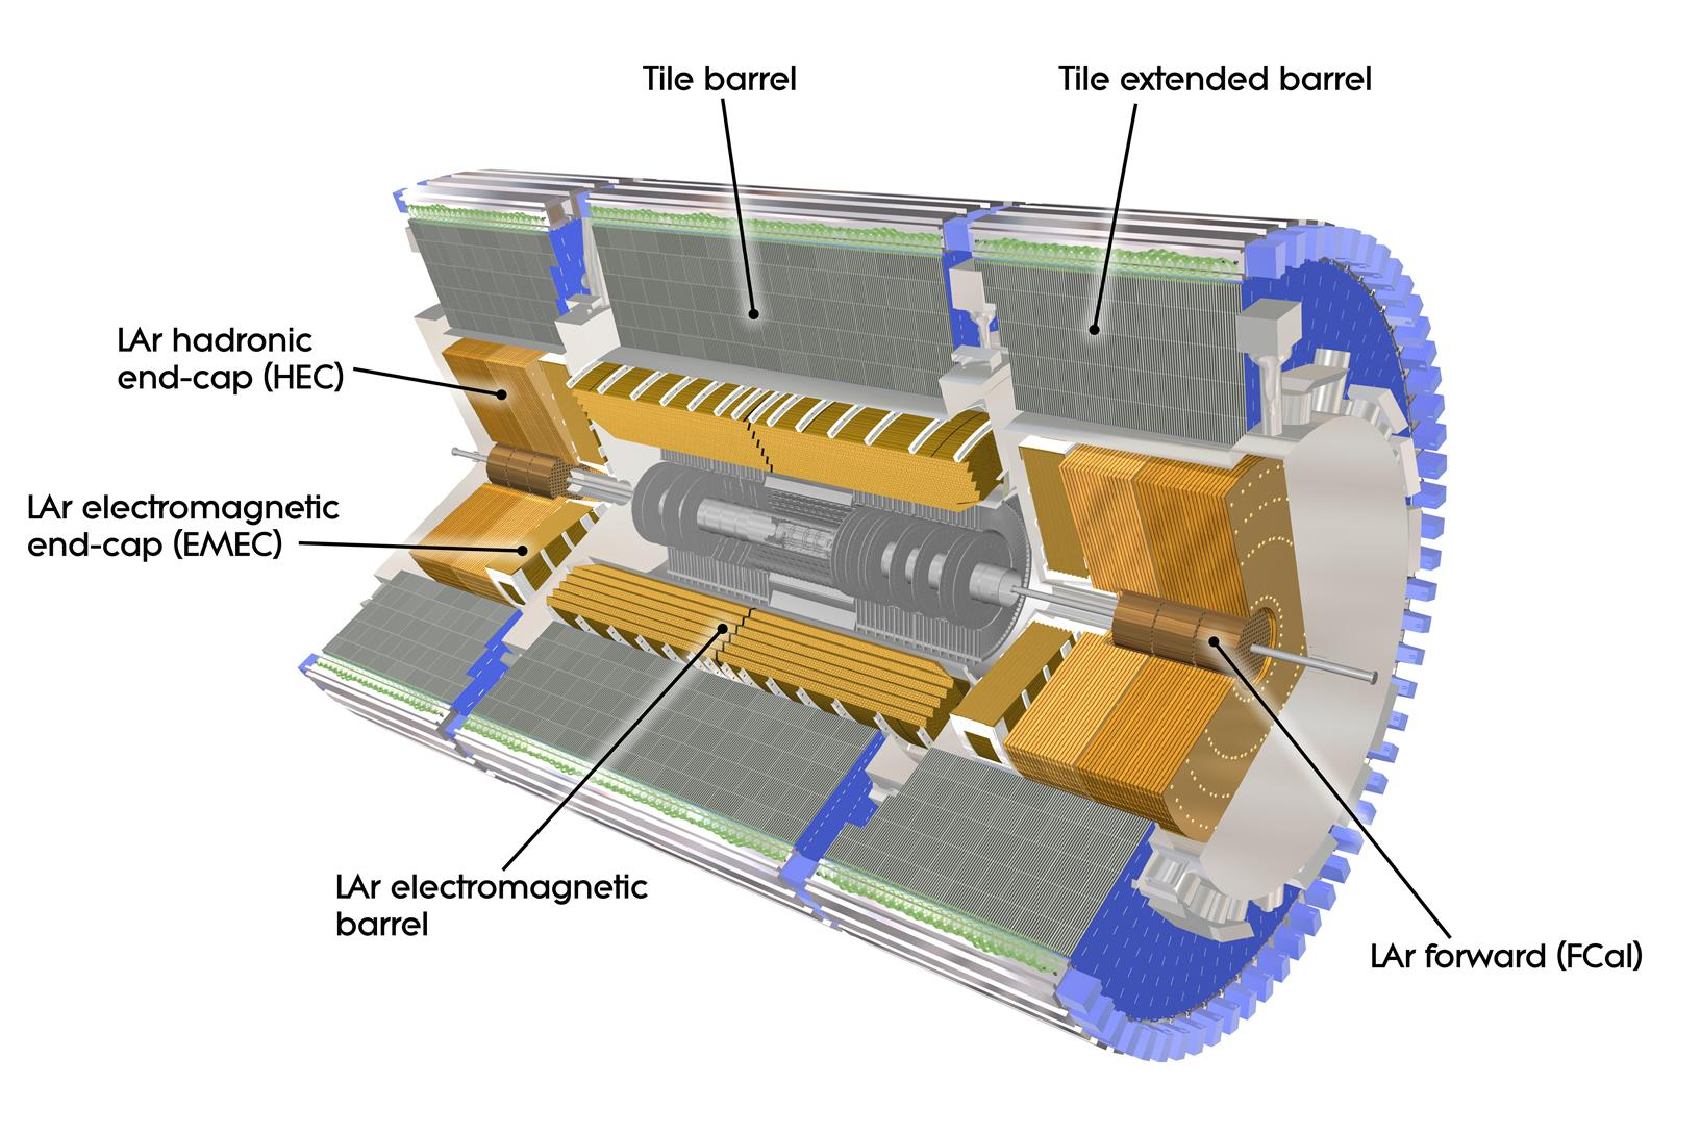
\includegraphics[width=0.75\textwidth]{figures/atlas/calorimeters}}
\caption{Layout of the ATLAS calorimeter system. Figure from Ref. \cite{atlas:atlas}}
\label{fig:atlas:calo}
\end{figure}

\subsubsection*{Electromagnetic Calorimeter}


\subsubsection*{Hadronic Calorimeter}


\subsubsection*{Forward Calorimeter}


\subsection{Muon Spectrometer}

\begin{figure}[ht]
\centering
\subfigure{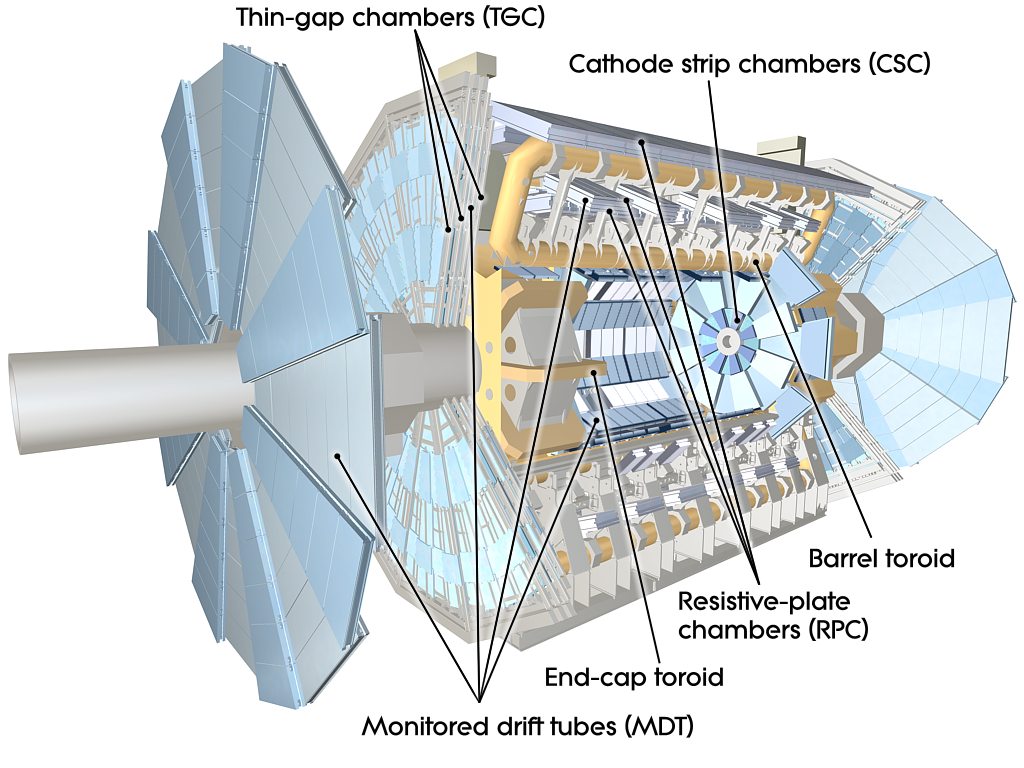
\includegraphics[width=0.65\textwidth]{figures/atlas/muon}}
\caption{Layout of the ATLAS muon system. Figure from Ref. \cite{atlas:atlas}}
\label{fig:atlas:muon}
\end{figure}

\subsection{Luminosity Detectors}

\subsection{Trigger System}
\label{sec:cern:trigger}

\subsection{ATLAS Performance Summary}


\subsection{ATLAS Physics Program}